\documentclass[a4paper, 12pt]{article}
\usepackage[utf8]{inputenc}
\renewcommand\familydefault{\sfdefault}
\usepackage[T1]{fontenc}
\usepackage[francais]{babel}
\usepackage[left=2cm,top=2cm,right=2cm,bottom=2cm]{geometry}
\usepackage{graphicx}
\usepackage{minted}
\usemintedstyle{colorful}
\usepackage{float}
\floatplacement{figure}{H}
\usepackage{authblk}
\usepackage{enumitem}
\usepackage{hyperref} 
\hypersetup{
	colorlinks,
	citecolor=black,
	filecolor=black,
	linkcolor=black,
	urlcolor=blue
}

\begin{document}

\title{Petits comptes entre amis} 
\author{Steven Liatti} 
\affil{\small Développement et services web - Prof. Stéphane Malandain} 
\affil{\small Hepia ITI 3\up{ème} année} 
\maketitle

\tableofcontents 
\listoffigures
\renewcommand\listoflistingscaption{Table des listings de code source}
\listoflistings

\section{Introduction}
\subsection{Description}
Le but de ce mini-projet est de réaliser un site en php permettant à des amis de noter et
partager les dépenses effectuées par et pour le groupe au cours de vacances
communes. Lorsque l’une des personnes fait des courses, par exemple, elle l’enregistre.
Chacun enregistre les dépenses qui concernent le groupe. Ainsi, à la fin du séjour (ou à
tout moment) on peut savoir qui a payé quoi et surtout ce que chacun doit aux autres
personnes du groupe d’amis.

\subsection{Technologies utilisées}
\begin{itemize}
	\item Base de données :
	\begin{itemize}
		\item \href{https://www.mysql.com/}{MySQL}, avec
		\item \href{https://www.mysql.com/products/workbench/}{MySQL Workbench} (pour la création du schéma)
	\end{itemize}
	\item Back-end :
	\begin{itemize}
		\item \href{https://httpd.apache.org/}{Apache}, serveur HTTP
		\item \href{http://php.net/}{PHP}, avec
		\item \href{https://silex.symfony.com/}{Silex}, micro framework PHP basé entre autres sur \href{https://symfony.com/}{Symfony}
	\end{itemize}
	\item Front-end :
	\begin{itemize}
		\item \href{https://twig.symfony.com/}{Twig}, moteur de templates pour PHP (utilisé de concert avec Silex)
		\item \href{https://jquery.org/}{jQuery}
		\item \href{http://getbootstrap.com/}{Bootstrap} pour le design en CSS
	\end{itemize}
\end{itemize}


\section{Base de données}
Les technologies imposées pour la base de données de ce travail pratique sont SQLite ou MySQL. J'ai choisi d'utiliser 
MySQL, car je suis familier avec. J'ai profité de cette occasion pour découvrir et utiliser Workbench, un programme 
permettant de modéliser les tables et relations d'une base de données de manière graphique. Une fois le model terminé, 
Workbench offre la possibilité de l'exporter en instructions SQL (création de tables et contraintes).
\bigbreak

Mon schéma est constitué des tables suivantes :
\begin{figure}
	\begin{center}
		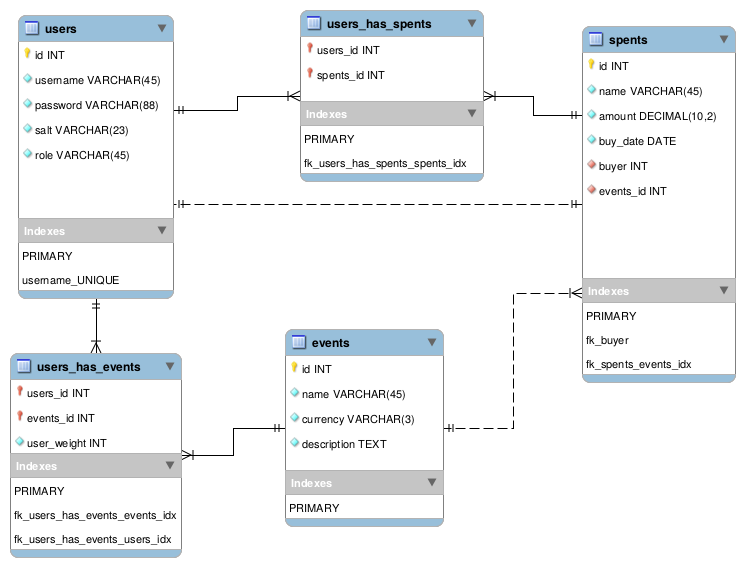
\includegraphics[width=1.0\textwidth]{database.png}
	\end{center}
	\caption{Schéma de la base de données relationnelle}
\end{figure}
Il y a 3 tables principales : les utilisateurs, les événements et les dépenses. 2 autres tables secondaires 
font la liaison entre les utilisateurs et les événements et les utilisateurs et les dépenses respectivement 
(liaison Many-To-Many). La table des utilisateurs possède un champ \mintinline{sql}{salt} et un autre 
\mintinline{sql}{role}, ils sont nécessaires au fonctionnement de Silex (explications plus loin). Le poids 
de chaque utilisateur au sein d'un événement est indiqué dans la table croisée 
\mintinline{sql}{users_has_events}. 
Chaque dépense référence l'acheteur (dans \mintinline{sql}{users}) et l'événement lié (dans \mintinline{sql}
{events}). Ce schéma représente l'interface minimum pour les données de ce travail, mais il a l'avantage 
d'être simple à comprendre et à maintenir.

\section{Back-end}
Je profite également de ce TP pour appréhender Silex, un micro framework PHP dérivé de Symfony (que j'ai eu 
l'occasion de tester), beaucoup plus léger que son grand frère mais tout de même robuste et modulaire. Il bénéficie 
d'un grand nombre de modules à ajouter, en vrac : système de templates, connexion à la base de données, routes, etc.

\subsection{Architecture MVC}
Grâce à Silex, mon architecture respecte le design pattern \href{https://en.wikipedia.org/wiki/Model-view-controller}{MVC}.
Voici l'arborescence du site :
\begin{figure}
	\begin{center}
		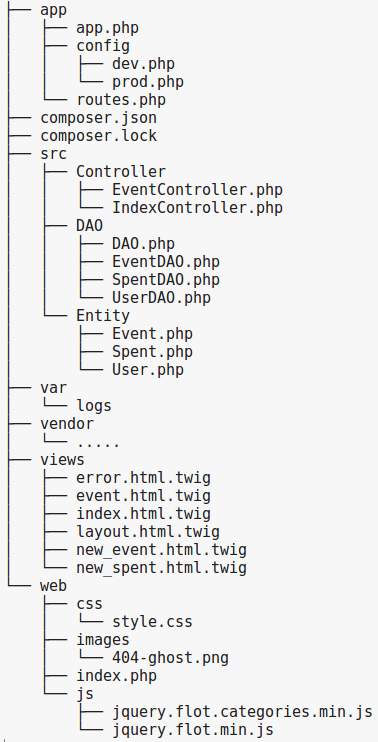
\includegraphics[width=0.5\textwidth]{tree.png}
	\end{center}
	\caption{Arborescence du site}
\end{figure}


\section{Front-end}



\section{Conclusion}
\subsection{État actuel du projet}

\subsection{Propositions d'améliorations}
\begin{itemize}
	\item Tests unitaires
	\item Dans une situation réelle de production, on ne laisserait pas un utilisateur choisir parmi tous les autres 
			utilisateurs au moment de créer un nouvel événement. Il faudrait plutôt ajouter des adresses email, 
			d'utilisateurs déjà inscrits (ou non) sur le site, ainsi chaque invité peut rejoindre l'événement.
	\item Changer le code lié à la sélection du poids de l'utilisateur (lors d'un nouvel évenement) pour l'intégrer 
			avec le composant Form de Symfony.
\end{itemize}


\end{document}
